\chapter[Trends]{Trends in observations and EMEP MSC-W model calculations 2000-2019}
\label{ch:Trends}

{\bf{Authors}}\\

\old{TODO}

\section{\label{sec:Trends_introduction}Introduction and background}
GP review bla bla


\section{\label{EMEPmodelcalc}{Setup for EMEP MSC-W model calculations}}
The EMEP MSC-W model version rv4.42 has been used for the all the model runs for years 2000 to 2019. The horizontal resolution is \resZO, with 20 vertical layers (the lowest with a height of approximately 50 meters).
 Meteorology, emissions, boundary conditions and forest fires for the respective years have been used as input. Meteorological data have been
 derived from ECMWF-IFS(cy40r1) simulations (see Section~\ref{sec:meteo}). 
 The boundary conditions for the main gaseous and aerosol species were based on climatological observed values with prescribed trends in trans-Atlantic fluxes, while the Mace
Head correction has been used for ozone. The boundary conditions for natural particles of
sea salt and mineral dust were the same as in the status run, namely 5-year monthly average
concentrations, derived from EMEP MSC-W global runs, kept invariable over the calculation
period.
Daily emissions from forest fires were from the Fire INventory from NCAR (FINN) for 2002-2016,
whereas for 2000 and 2001 (unavailable from FINN), monthly averages over 2005-2015 were
used.
 Volcanic emissions...?
 
 OC/EC split
 NMVOC split
 
A revised set of emissions for all the years 2000-2019 have been used in the model calculations (including all the reported and re-reported data by summer 2021), see chapter \ref{ch:emis2019}.

\section{\label{OBSTrends}{Observations}} NILU to write

\section{\label{Method}{Method for calculation of trends}}
Both observed and modelled trends were processed with the pyaerocom software (\url{https://github.com/metno/pyaerocom}, version XXX) for the following periods: 2000-2019, 2000-2010, 2010-2019, and 2005-2019. All observations were provided via the EBAS database. 

In order to compute trends, for each station and variable, time series data was merged in time to cover the respective time period for the trends.
Since the provided temporal resolution can change over time for a given site, the lowest common resolution was identified and higher resolution data were down-sampled to that resolution during the merging process. For temporal re-sampling, a conservative scheme was used requiring ca 75\% coverage in a hierarchical manner, that is, at least 18 hourly measurement values to retrieve a daily mean, and at least 21 daily values to retrieve a monthly mean. Trends are computed based on yearly averages, as described in more details below. To retrieve the yearly averages, at least one monthly value is required per season. In addition to trends based on yearly averages, seasonal trends are computed as well for all variables but O$_{3}$ which is focusing on the summer maximum using percentiles (details below). In addition to this conservative re-sampling scheme, a second analysis was done using 25\% coverage constraint instead of 75\% coverage. Finally, a minimum number of yearly averages was required to be available for the trends computation depending on the length of the period, corresponding to ca 75\% (e.g. 14 yearly values for the period 2000-2019).

For O$_3$, the re-sampling was done differently, that is, daily max values were computed based on hourly measurements, requiring at least 18 hourly measurements per day as for the other variables. Then, the yearly average was computed using different percentiles of the daily values (10, 50, 75, 95, 98, 99 percentiles), requiring at least 330 daily max values in a given year. Trends were then computed for each of these percentile averages.

Model output is given on daily resolution, including the daily max O$_3$. To compute the model trends, the model output for each variable was collocated in space and time with the observations. Collocation in space was done by picking the nearest model grid to each station. Collocation in time was done by first re-sampling both model and observation data to the lowest common temporal resolution, then invalidating the model output at times when observations are missing, and finally calculating the monthly mean of both. Precipitation (reported in units of mm) was collocated in time based on monthly aggregates, which were calculated independently for model and observations.

The monthly time series of the collocated model and observation data were output as csv files for each individual site. The scripts used for processing the data and calculating trends are available from a GitHub repository (\url{https://github.com/metno/emep_trends_2021}). The processed data itself, including relevant station metadata and trends results, are available in a separate location which is linked to in the description of the repository.

The same methodology as described by \cite{aas2019global, mortier2020} has been used to derive the trends at the individual stations. The significance of the trends is tested with the Mann-Kendall test \citep{hamed1998modified}. The related p-value is used to determine if the trend is significant or not within a confidence interval of 68 \%. The slope is calculated with the Theil-Sen estimator which is less sensitive to outliers than standard least-squares methods \citep{sen1968estimates}.

An uncertainty is provided for each trend by combining the error of the slope calculation itself to the error of the residuals:

\begin{equation}
 Uncertainty = \sqrt{{\left (\frac{\Delta m}{y(start)}\right )}^{2} + {\left ( \frac{m \cdot \Delta r}{y(start)^2}\right )}^{2} }
\end{equation}

where $\Delta m$ is the Theil-Sen estimator 95\% confidence interval, $y(start)$ is the value of the regression line at the first year of the period, $m$ is the value of the Theil-Sen slope and $\Delta r$ is the averaged error on the residuals computed based on the difference between the linear trend and the yearly mean values of the regional time series.

In order to allow for consistent comparisons, the trend is provided as a relative trend (\%/yr) with respect to the first year of the time period.



\section{\label{sec:Trends_sulfur}Trends in sulfur}

Figure~\ref{fig:SOx_trends} shows an overview of the annual and seasonal trends in oxidised sulfur compounds from 2000 to 2019.

\begin{figure}
	\centering
	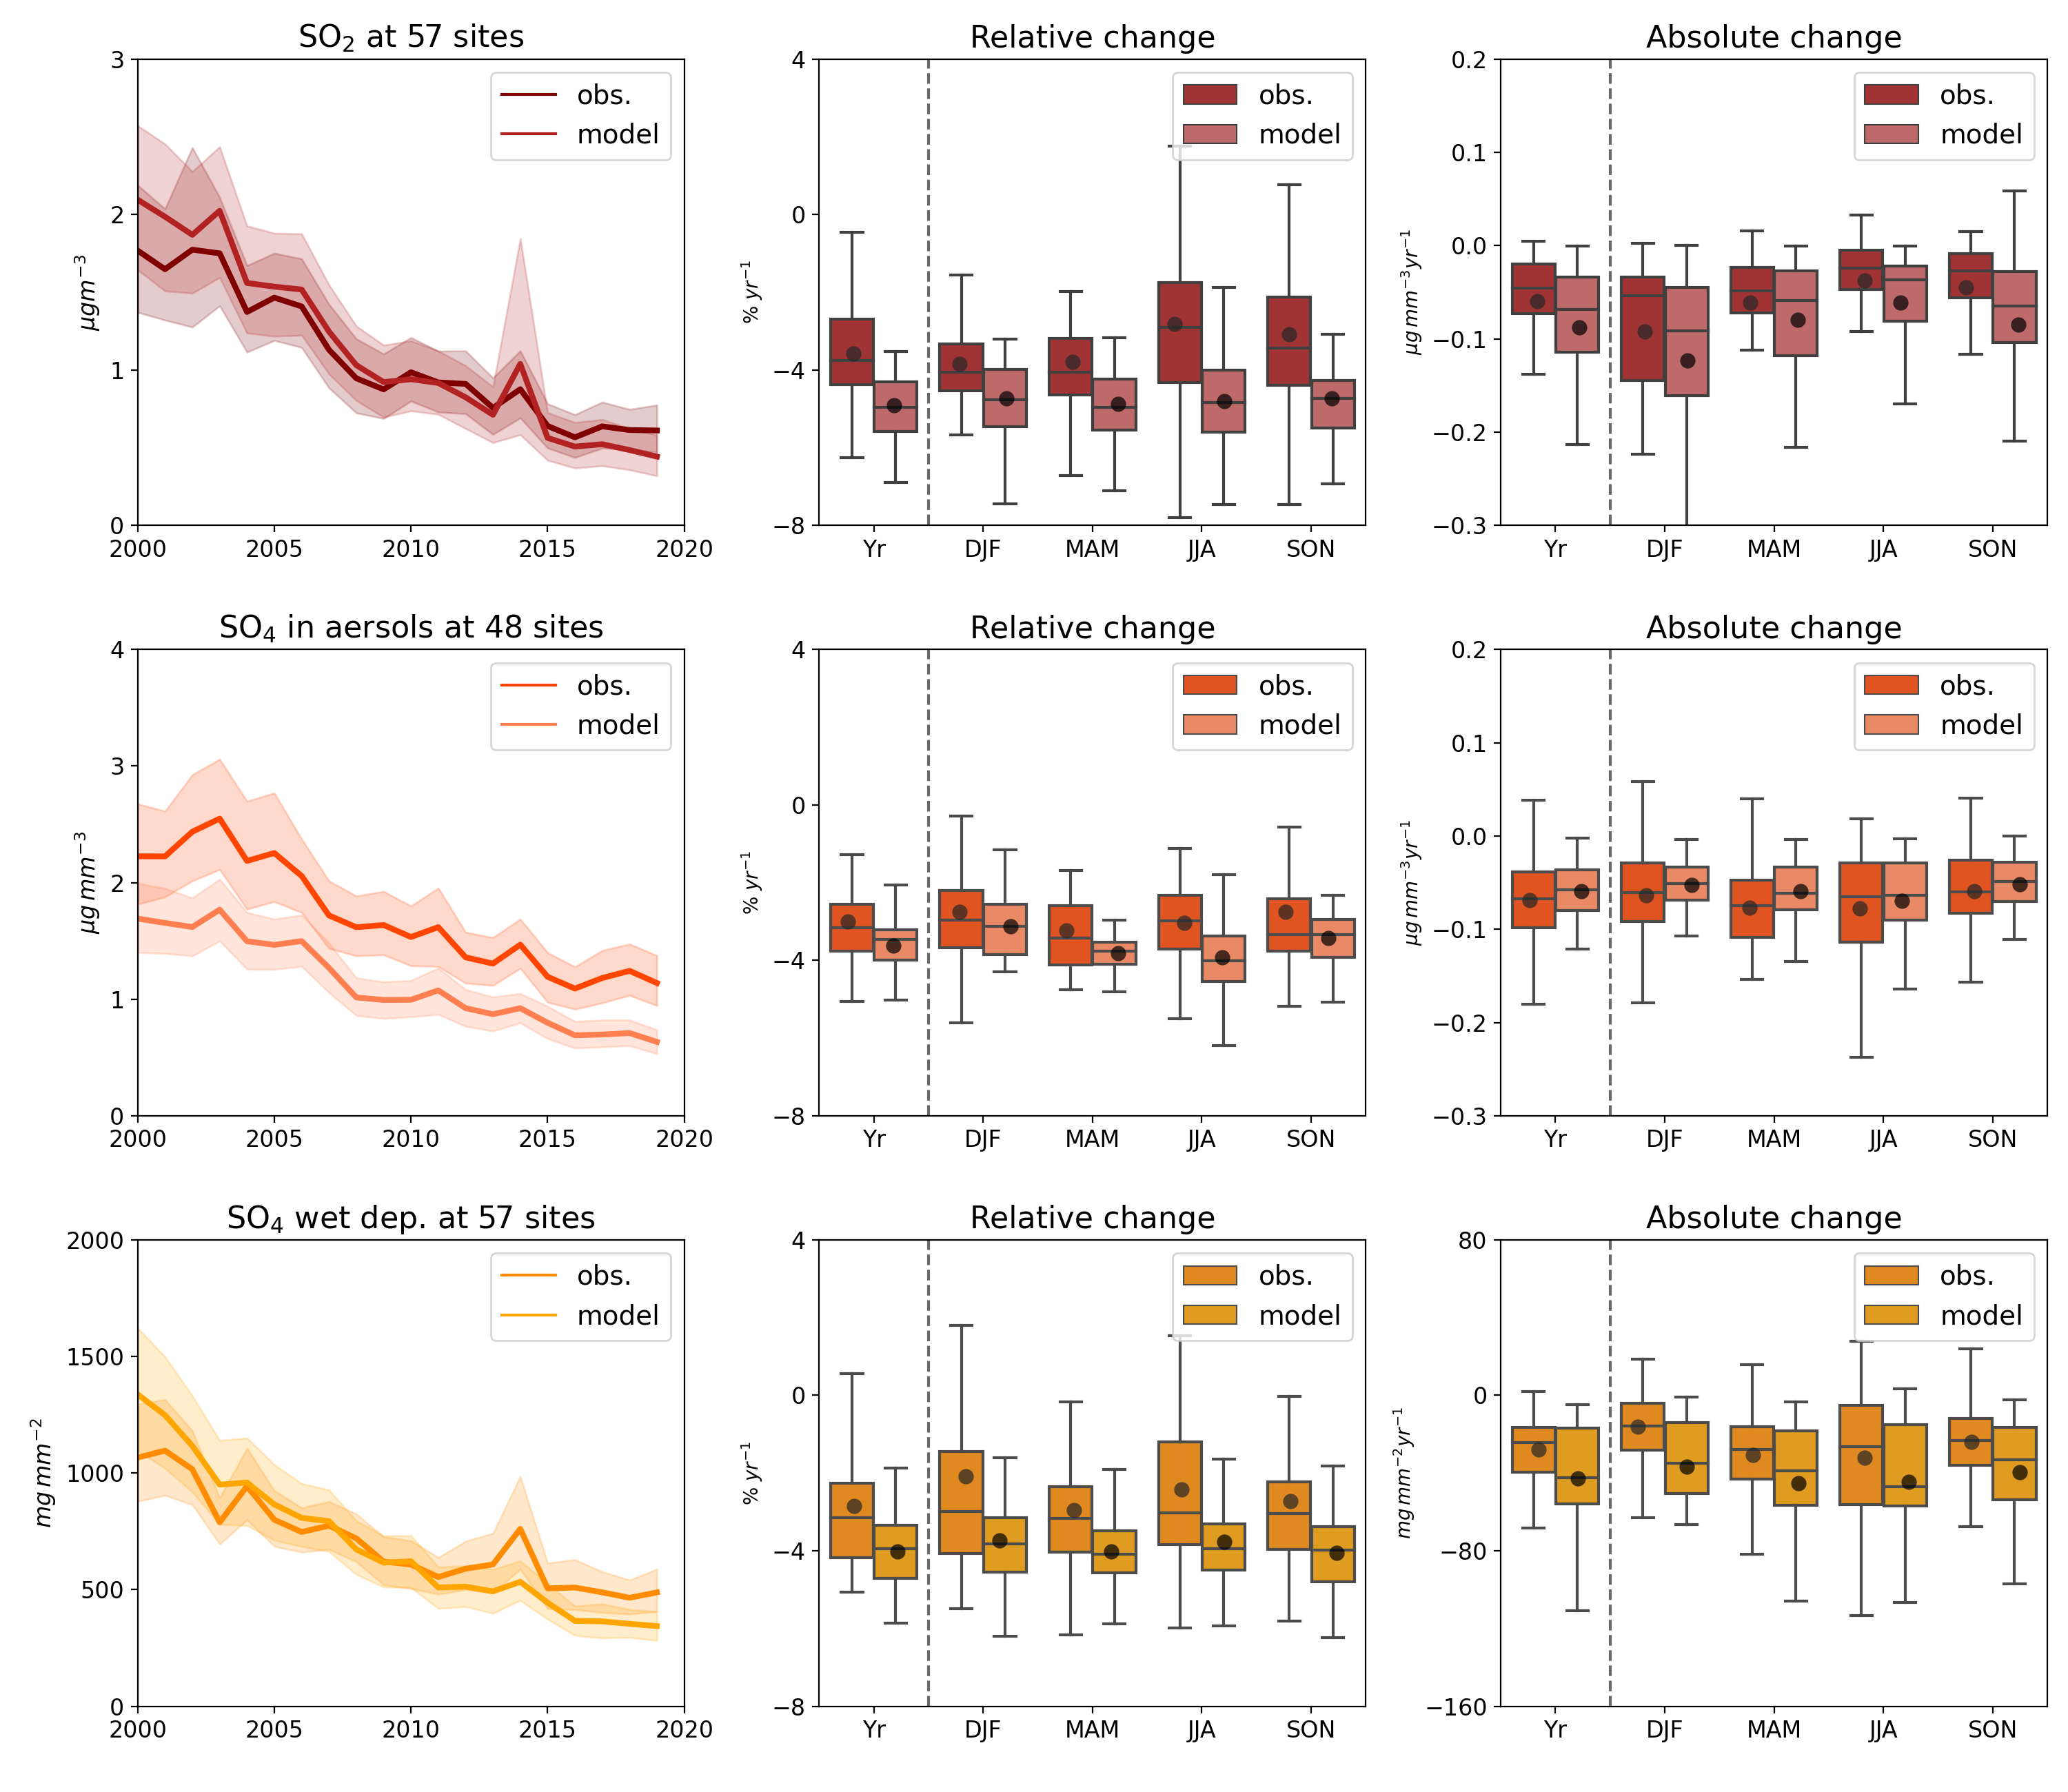
\includegraphics[width=0.74\paperwidth]{FIGS_TRENDS/sulfur_trends.png}
	\caption{\label{fig:SOx_trends}Trends in sulfur components from 2010-2019 for EMEP observations and model.}
\end{figure}

\begin{table}
\caption{\label{tab:so2_stat} Average absolute and relative changes in \soii concentrations}
\begin{center}
\scalebox{0.65}{%
\begin{tabular}{ll|ccc|cccc|cccc}
\toprule
          &        & \multicolumn{3}{c}{Number of sites} & \multicolumn{4}{c}{Average change per year (\ug $yr^{-1})$} & \multicolumn{4}{c}{Relative change per year (\% $yr^{-1}$)} \\
Period & Seasons &           total & sign.(obs.) & sign.(mod.) &                    obs. &          conf.interval &  mod. &          conf.interval &                     obs. &         conf.interval &  mod. &        conf.interval \\
\midrule
2000-2019 & all &              57 &          50 &          55 &                  -0.060 &  (-0.075, -0.045) & -0.088 &  (-0.108, -0.068) &                    -3.59 &   (-3.98, -3.2) & -4.91 &  (-5.27, -4.54) \\
          & autumn &              57 &          38 &          53 &                  -0.045 &  (-0.059, -0.031) & -0.085 &  (-0.106, -0.063) &                    -3.09 &   (-3.68, -2.5) & -4.73 &  (-5.18, -4.27) \\
          & spring &              57 &          50 &          54 &                  -0.061 &  (-0.076, -0.046) & -0.080 &  (-0.099, -0.061) &                    -3.80 &  (-4.18, -3.42) & -4.88 &  (-5.22, -4.54) \\
          & summer &              57 &          37 &          56 &                  -0.038 &   (-0.05, -0.025) & -0.062 &  (-0.079, -0.044) &                    -2.82 &  (-3.37, -2.27) & -4.81 &   (-5.2, -4.42) \\
          & winter &              59 &          49 &          55 &                  -0.092 &  (-0.115, -0.069) & -0.123 &   (-0.15, -0.095) &                    -3.85 &   (-4.2, -3.51) & -4.73 &  (-5.09, -4.36) \\
2005-2019 & all &              68 &          45 &          62 &                  -0.062 &   (-0.09, -0.033) & -0.067 &  (-0.083, -0.052) &                    -3.82 &  (-4.41, -3.24) & -5.08 &  (-5.44, -4.72) \\
2010-2019 & all &              73 &          40 &          48 &                  -0.047 &   (-0.063, -0.03) & -0.063 &  (-0.079, -0.047) &                    -4.07 &  (-5.19, -2.96) & -6.13 &  (-6.94, -5.32) \\
2000-2010 & all &              77 &          36 &          66 &                  -0.075 &  (-0.097, -0.053) & -0.115 &  (-0.139, -0.091) &                    -3.61 &  (-4.39, -2.82) & -5.33 &   (-5.85, -4.8) \\
\bottomrule
\end{tabular}}
\end{center}
\end{table}

\begin{table}
\caption{\label{tab:so4pm_stat} Average absolute and relative changes in \soiv concentrations in aerosols}
\begin{center}
\scalebox{0.65}{%
\begin{tabular}{ll|ccc|cccc|cccc}
\toprule
          &        & \multicolumn{3}{c}{Number of sites} & \multicolumn{4}{c}{Average change per year (\ug $yr^{-1})$} & \multicolumn{4}{c}{Relative change per year (\% $yr^{-1}$)} \\
Period & Seasons &           total & sign.(obs.) & sign.(mod.) &                    obs. &          conf.interval &  mod. &          conf.interval &                     obs. &         conf.interval &  mod. &        conf.interval \\
\midrule
2000-2019 & all &              48 &          46 &          48 &                  -0.069 &  (-0.082, -0.056) & -0.059 &  (-0.069, -0.049) &                    -3.00 &  (-3.36, -2.65) & -3.63 &  (-3.87, -3.39) \\
          & autumn &              46 &          40 &          45 &                  -0.059 &  (-0.074, -0.044) & -0.052 &  (-0.061, -0.043) &                    -2.76 &  (-3.42, -2.09) & -3.43 &   (-3.67, -3.2) \\
          & spring &              47 &          44 &          47 &                  -0.077 &   (-0.09, -0.064) & -0.059 &   (-0.068, -0.05) &                    -3.23 &  (-3.58, -2.87) & -3.82 &  (-4.02, -3.61) \\
          & summer &              47 &          43 &          46 &                  -0.077 &   (-0.095, -0.06) & -0.070 &  (-0.085, -0.054) &                    -3.03 &  (-3.36, -2.71) & -3.93 &  (-4.25, -3.61) \\
          & winter &              49 &          36 &          40 &                  -0.064 &  (-0.081, -0.046) & -0.052 &  (-0.061, -0.044) &                    -2.75 &  (-3.24, -2.27) & -3.12 &   (-3.35, -2.9) \\
2005-2019 & all &              53 &          42 &          48 &                  -0.060 &  (-0.072, -0.047) & -0.049 &  (-0.057, -0.041) &                    -3.14 &  (-3.74, -2.54) & -3.67 &  (-3.97, -3.37) \\
2010-2019 & all &              58 &          23 &          37 &                  -0.046 &  (-0.059, -0.032) & -0.044 &  (-0.054, -0.033) &                    -3.08 &  (-3.73, -2.42) & -4.01 &  (-4.63, -3.39) \\
2000-2010 & all &              70 &          24 &          48 &                  -0.067 &  (-0.097, -0.037) & -0.081 &  (-0.094, -0.069) &                    -1.83 &  (-2.79, -0.86) & -3.90 &  (-4.24, -3.57) \\
\bottomrule
\end{tabular}}
\end{center}
\end{table}

\begin{table}
\caption{\label{tab:so4dep_stat} Average absolute and relative changes in wet deposition of sulfate}
\begin{center}
\scalebox{0.65}{%
\begin{tabular}{ll|ccc|cccc|cccc}
\toprule
          &        & \multicolumn{3}{c}{Number of sites} & \multicolumn{4}{c}{Average change per year (mg $mm^{2} yr^{-1}$)} & \multicolumn{4}{c}{Relative change per year (\% $yr^{-1}$)} \\
Period & Seasons &           total & sign.(obs.) & sign.(mod.) &                    obs. &          conf.interval &  mod. &          conf.interval &                     obs. &         conf.interval &  mod. &        conf.interval \\
\midrule
2000-2019 & all &              57 &          43 &          56 &                   -27.8 &  (-32.9, -22.6) & -42.7 &  (-50.7, -34.6) &                    -2.85 &  (-3.31, -2.38) & -4.01 &  (-4.27, -3.75) \\
          & autumn &              54 &          28 &          47 &                   -24.0 &  (-29.4, -18.6) & -39.6 &  (-48.4, -30.8) &                    -2.72 &  (-3.26, -2.18) & -4.06 &  (-4.36, -3.75) \\
          & spring &              53 &          32 &          52 &                   -30.9 &  (-36.8, -24.9) & -45.4 &  (-55.3, -35.5) &                    -2.96 &  (-3.39, -2.52) & -4.02 &  (-4.25, -3.79) \\
          & summer &              55 &          33 &          49 &                   -32.3 &  (-40.2, -24.3) & -44.5 &  (-53.8, -35.2) &                    -2.42 &  (-2.98, -1.87) & -3.78 &  (-4.11, -3.44) \\
          & winter &              56 &          27 &          50 &                   -16.1 &   (-23.3, -8.8) & -36.7 &  (-44.0, -29.4) &                    -2.08 &  (-3.05, -1.12) & -3.74 &  (-4.02, -3.46) \\
2005-2019 & all &              62 &          31 &          53 &                   -21.6 &  (-26.5, -16.7) & -31.2 &  (-36.8, -25.5) &                    -2.61 &  (-3.25, -1.97) & -4.04 &  (-4.35, -3.73) \\
2010-2019 & all &              74 &          15 &          40 &                   -19.2 &  (-26.0, -12.4) & -31.7 &  (-38.6, -24.8) &                    -1.95 &  (-3.16, -0.74) & -4.58 &   (-5.1, -4.05) \\
2000-2010 & all &              66 &          29 &          43 &                   -45.8 &  (-55.2, -36.5) & -58.6 &  (-70.2, -47.0) &                    -4.14 &  (-4.85, -3.42) & -4.87 &  (-5.34, -4.39) \\
\bottomrule
\end{tabular}}
\end{center}
\end{table}


\section{\label{sec:Trends_oxidised_nitrogen }Trends in oxidised nitrogen}

Figure~\ref{fig:NOx_trends} shows an overview of the annual and seasonal trends in oxidised nitrogen compounds from 2000 to 2019.

\begin{figure}
	\centering
	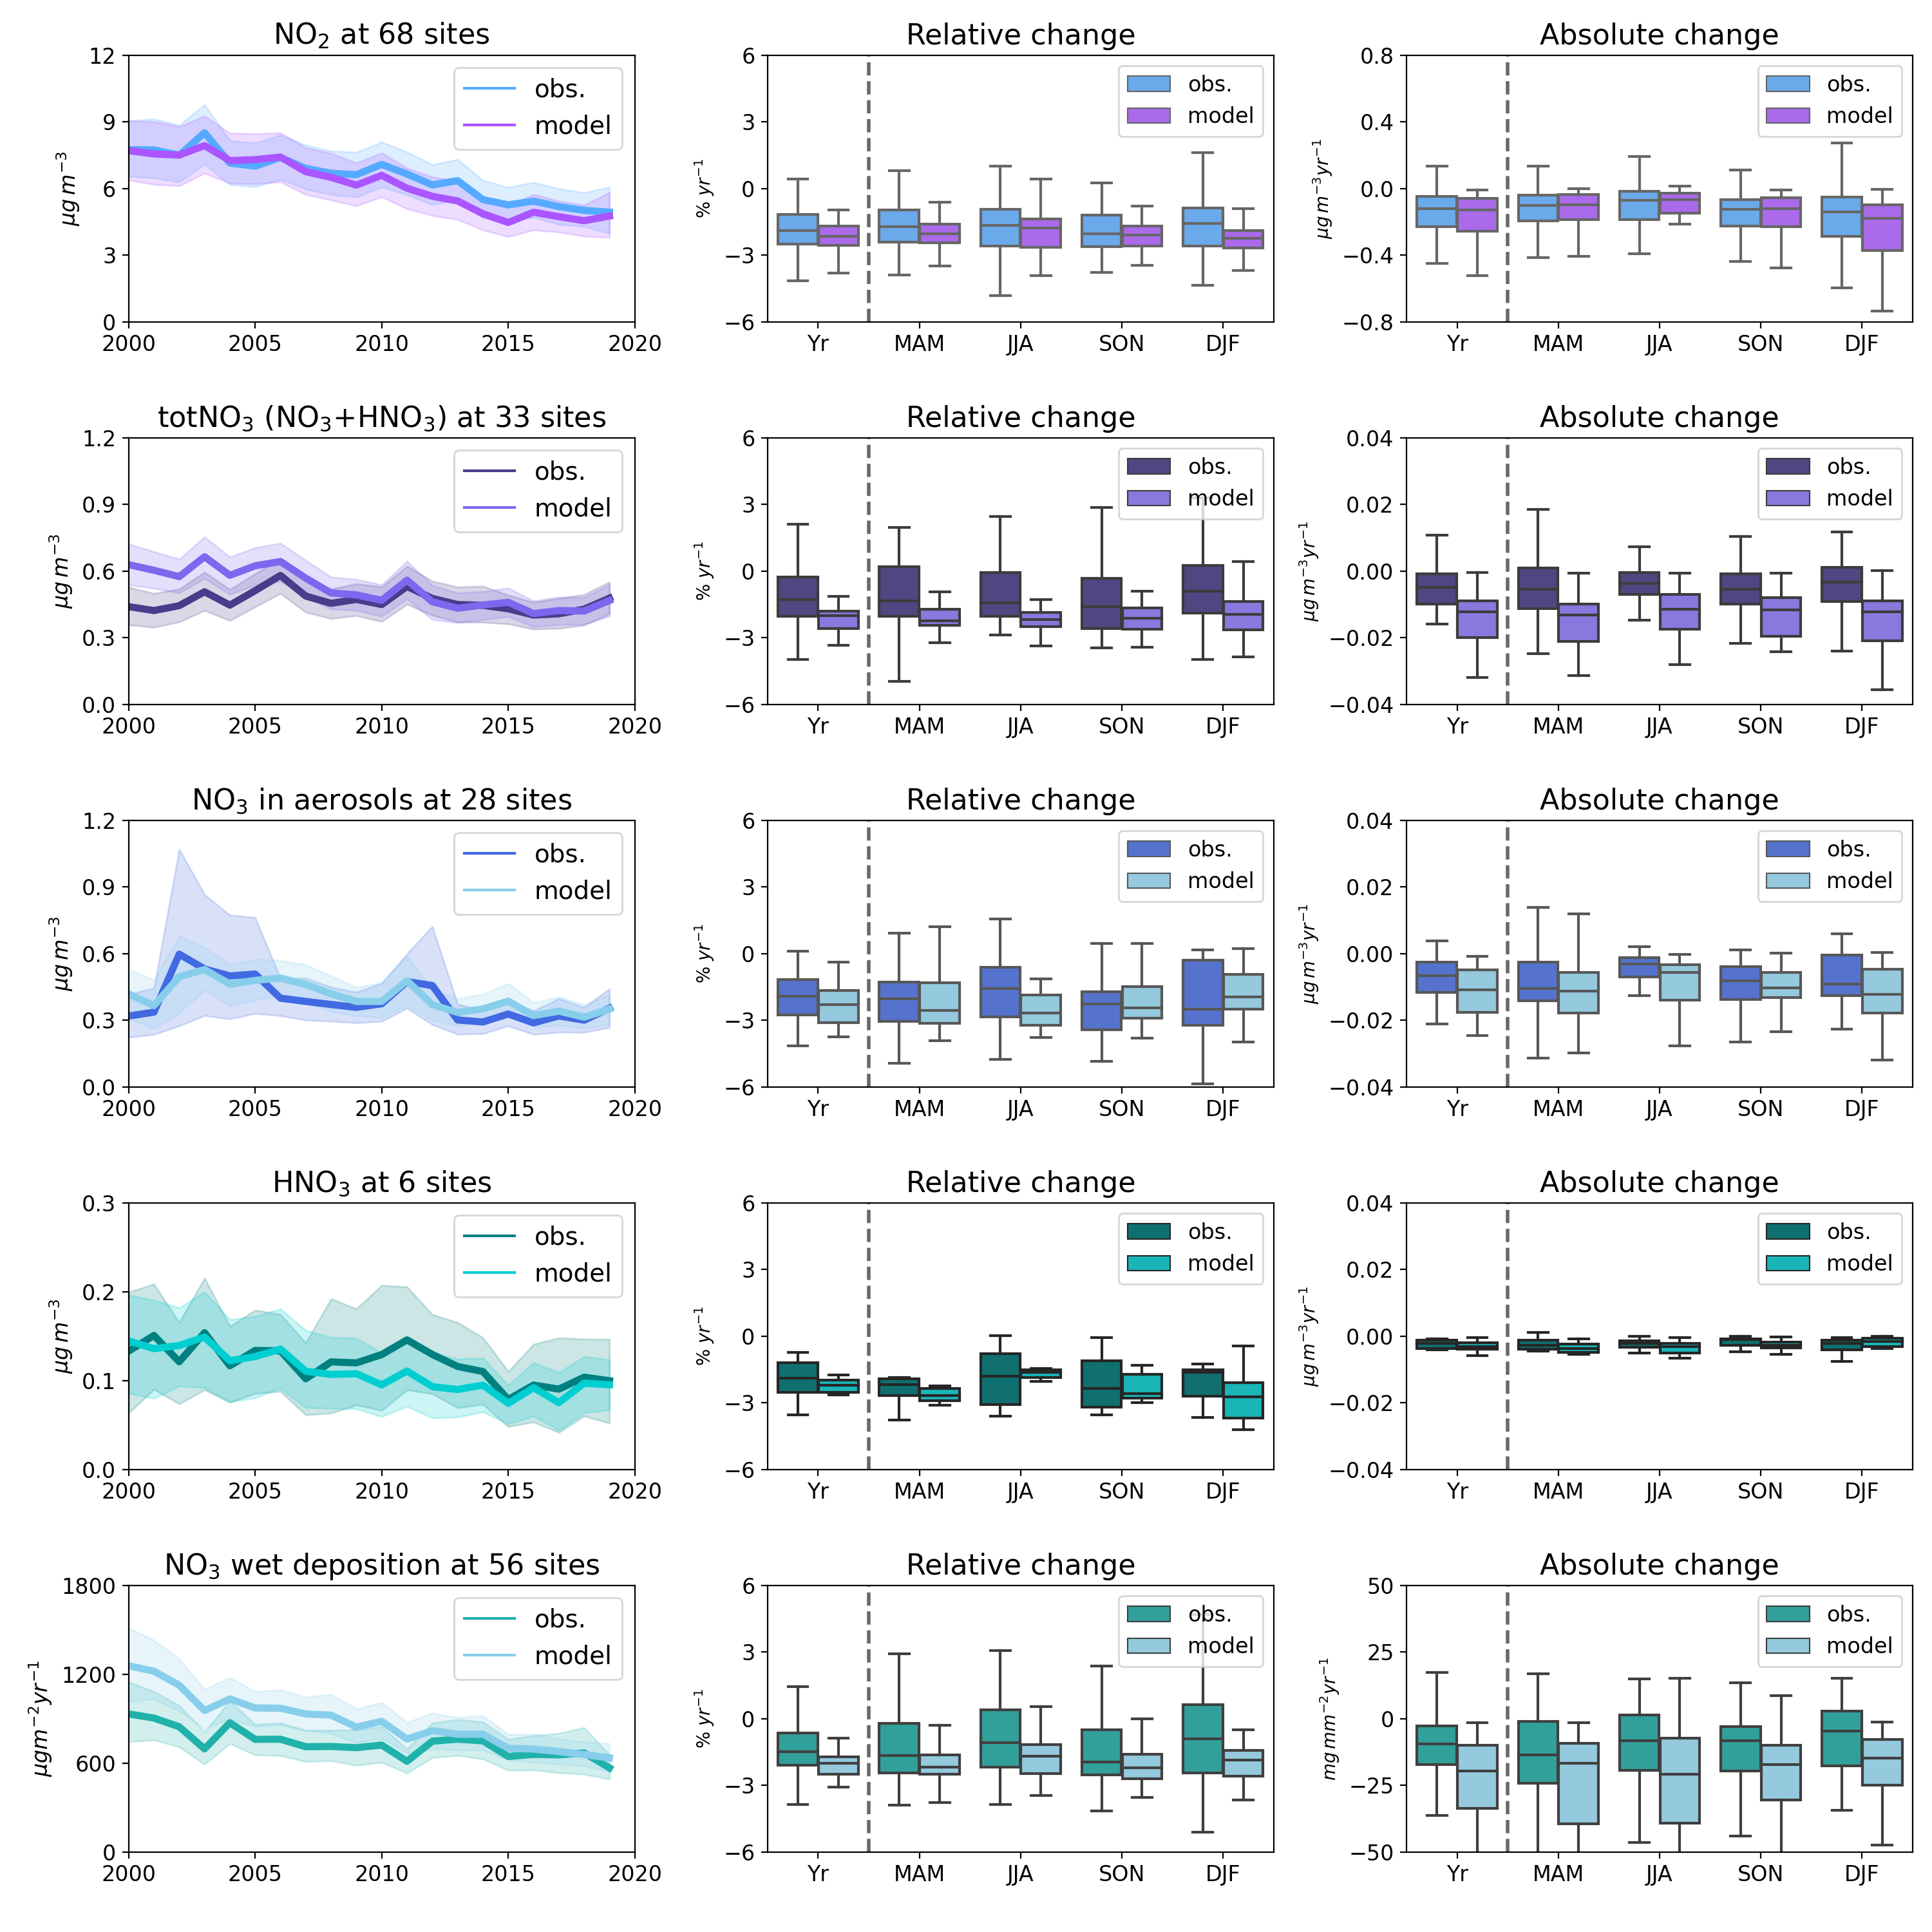
\includegraphics[width=0.74\paperwidth]{FIGS_TRENDS/Nox_trends.png}
	\caption{\label{fig:NOx_trends}Trends in oxidised nitrogen compounds from 2010-2019 for EMEP observations and model.}
\end{figure}


\begin{table}
\caption{\label{tab:no2_stat} Average absolute and relative changes in \noii concentrations}
\begin{center}
\scalebox{0.65}{%
\begin{tabular}{ll|ccc|cccc|cccc}
\toprule
          &        & \multicolumn{3}{c}{Number of sites} & \multicolumn{4}{c}{Average change per year (\ug $yr^{-1})$} & \multicolumn{4}{c}{Relative change per year (\% $yr^{-1}$)} \\
Period & Seasons &           total & sign.(obs.) & sign.(mod.) &                    obs. &          conf.interval &  mod. &          conf.interval &                     obs. &         conf.interval &  mod. &        conf.interval \\
\midrule
2000-2019 & all &              68 &          48 &          67 &                  -0.135 &  (-0.166, -0.105) & -0.191 &  (-0.233, -0.149) &                    -1.24 &  (-2.15, -0.33) & -2.22 &  (-2.38, -2.06) \\
          & autumn &              67 &          43 &          66 &                  -0.146 &   (-0.18, -0.113) & -0.192 &  (-0.237, -0.147) &                    -1.19 &  (-2.32, -0.06) & -2.19 &  (-2.35, -2.02) \\
          & spring &              67 &          38 &          63 &                  -0.124 &  (-0.155, -0.093) & -0.156 &  (-0.196, -0.116) &                    -0.96 &    (-2.03, 0.1) & -2.02 &   (-2.2, -1.84) \\
          & summer &              67 &          43 &          63 &                  -0.101 &  (-0.128, -0.074) & -0.135 &  (-0.175, -0.095) &                    -1.24 &  (-2.03, -0.44) & -1.87 &   (-2.1, -1.65) \\
          & winter &              69 &          33 &          65 &                  -0.151 &  (-0.189, -0.114) & -0.253 &  (-0.297, -0.208) &                    -1.17 &  (-1.97, -0.36) & -2.34 &  (-2.49, -2.18) \\
2005-2019 & all &              75 &          53 &          71 &                  -0.151 &   (-0.183, -0.12) & -0.193 &  (-0.234, -0.152) &                    -1.84 &  (-2.47, -1.21) & -2.57 &  (-2.77, -2.37) \\
2010-2019 & all &              79 &          39 &          56 &                  -0.152 &   (-0.194, -0.11) & -0.162 &  (-0.199, -0.125) &                    -2.27 &  (-3.05, -1.49) & -2.39 &  (-2.69, -2.09) \\
2000-2010 & all &              76 &          12 &          44 &                  -0.098 &  (-0.144, -0.052) & -0.161 &  (-0.207, -0.116) &                    -0.95 &  (-1.67, -0.24) & -1.73 &  (-2.07, -1.39) \\
\bottomrule
\end{tabular}}
\end{center}
\end{table}


\begin{table}
\caption{\label{tab:tno3_stat} Average absolute and relative changes in  concentration of total nitrate ({\ensuremath{\mbox{HNO}_{\rm 3}}} + \noiii) in air and aerosols}
\begin{center}
\scalebox{0.65}{%
\begin{tabular}{ll|ccc|cccc|cccc}
\toprule
          &        & \multicolumn{3}{c}{Number of sites} & \multicolumn{4}{c}{Average change per year (\ug $yr^{-1})$} & \multicolumn{4}{c}{Relative change per year (\% $yr^{-1}$)} \\
Period & Seasons &           total & sign.(obs.) & sign.(mod.) &                    obs. &          conf.interval &  mod. &          conf.interval &                     obs. &         conf.interval &  mod. &        conf.interval \\
\midrule
2000-2019 & all &              33 &          18 &          32 &                  -0.005 &  (-0.008, -0.002) & -0.013 &  (-0.016, -0.011) &                    -0.79 &  (-1.55, -0.04) & -2.10 &  (-2.28, -1.92) \\
          & autumn &              32 &          17 &          22 &                  -0.006 &   (-0.01, -0.002) & -0.014 &  (-0.017, -0.011) &                    -0.96 &   (-1.91, -0.0) & -2.14 &  (-2.36, -1.92) \\
          & spring &              33 &          14 &          29 &                  -0.006 &  (-0.009, -0.002) & -0.014 &  (-0.017, -0.012) &                    -0.74 &   (-1.53, 0.04) & -2.12 &   (-2.33, -1.9) \\
          & summer &              33 &          18 &          29 &                  -0.003 &  (-0.005, -0.001) & -0.012 &   (-0.015, -0.01) &                    -0.87 &   (-1.45, -0.3) & -2.14 &  (-2.31, -1.97) \\
          & winter &              35 &           8 &          24 &                  -0.004 &   (-0.009, 0.001) & -0.015 &  (-0.019, -0.012) &                    -0.02 &   (-1.17, 1.13) & -2.02 &   (-2.3, -1.73) \\
2005-2019 & all &              39 &          23 &          33 &                  -0.010 &  (-0.013, -0.008) & -0.014 &  (-0.017, -0.012) &                    -2.04 &   (-2.68, -1.4) & -2.46 &  (-2.72, -2.21) \\
2010-2019 & all &              38 &          20 &          10 &                  -0.010 &  (-0.017, -0.003) & -0.010 &  (-0.013, -0.008) &                    -2.25 &  (-3.64, -0.86) & -2.03 &  (-2.36, -1.71) \\
2000-2010 & all &              46 &          14 &          16 &                   0.002 &   (-0.005, 0.009) & -0.015 &  (-0.019, -0.012) &                     2.20 &     (0.2, 4.19) & -1.99 &  (-2.46, -1.52) \\
\bottomrule
\end{tabular}}
\end{center}
\end{table}

\begin{table}
\caption{\label{tab:no3pm_stat} Average absolute and relative changes in \noiii concentrations in aerosols}
\begin{center}
\scalebox{0.65}{%
\begin{tabular}{ll|ccc|cccc|cccc}
\toprule
          &        & \multicolumn{3}{c}{Number of sites} & \multicolumn{4}{c}{Average change per year (\ug $yr^{-1})$} & \multicolumn{4}{c}{Relative change per year (\% $yr^{-1}$)} \\
Period & Seasons &           total & sign.(obs.) & sign.(mod.) &                    obs. &          conf.interval &  mod. &          conf.interval &                     obs. &         conf.interval &  mod. &        conf.interval \\
\midrule
2000-2019 & all &              28 &          18 &          20 &                  -0.009 &  (-0.013, -0.005) & -0.012 &  (-0.016, -0.008) &                    -1.64 &   (-2.63, -0.66) & -2.19 &  (-2.49, -1.88) \\
          & autumn &              27 &          15 &          13 &                  -0.010 &  (-0.016, -0.005) & -0.012 &  (-0.017, -0.007) &                    -1.92 &    (-3.24, -0.6) & -2.15 &  (-2.55, -1.75) \\
          & spring &              27 &          17 &          18 &                  -0.011 &  (-0.016, -0.005) & -0.011 &  (-0.015, -0.007) &                    -1.63 &   (-2.58, -0.67) & -1.93 &  (-2.56, -1.29) \\
          & summer &              27 &          12 &          17 &                  -0.004 &  (-0.006, -0.002) & -0.009 &  (-0.012, -0.006) &                    -1.41 &   (-2.23, -0.58) & -2.41 &   (-2.7, -2.12) \\
          & winter &              30 &          15 &           7 &                  -0.010 &   (-0.023, 0.003) & -0.012 &  (-0.015, -0.009) &                    -0.52 &    (-2.29, 1.24) & -1.65 &  (-2.15, -1.15) \\
2005-2019 & all &              39 &          16 &          23 &                  -0.009 &  (-0.013, -0.006) & -0.011 &  (-0.015, -0.007) &                    -2.12 &   (-3.06, -1.18) & -2.10 &  (-2.86, -1.33) \\
2010-2019 & all &              48 &           5 &          10 &                  -0.002 &   (-0.011, 0.008) & -0.007 &  (-0.011, -0.004) &                    -0.51 &    (-2.47, 1.44) & -1.09 &  (-1.84, -0.35) \\
2000-2010 & all &              38 &           8 &          16 &                  -0.017 &    (-0.04, 0.007) & -0.017 &  (-0.023, -0.012) &                    -1.47 &     (-3.2, 0.27) & -2.55 &  (-3.19, -1.91) \\
\bottomrule
\end{tabular}}
\end{center}
\end{table}

\begin{table}
\caption{\label{tab:hno3_stat} Average absolute and relative changes in {\ensuremath{\mbox{HNO}_{\rm 3}}} concentrations}
\begin{center}
\scalebox{0.65}{%
\begin{tabular}{ll|ccc|cccc|cccc}
\toprule
          &        & \multicolumn{3}{c}{Number of sites} & \multicolumn{4}{c}{Average change per year (\ug $yr^{-1})$} & \multicolumn{4}{c}{Relative change per year (\% $yr^{-1}$)} \\
Period & Seasons &           total & sign.(obs.) & sign.(mod.) &                    obs. &          conf.interval &  mod. &          conf.interval &                     obs. &         conf.interval &  mod. &        conf.interval \\
\midrule
2000-2019 & all &               6 &           4 &           6 &                  -0.002 &  (-0.004, -0.001) & -0.003 &  (-0.005, -0.002) &                    -1.94 &  (-2.77, -1.11) & -2.24 &  (-2.53, -1.95) \\
          & autumn &               6 &           3 &           6 &                  -0.002 &    (-0.003, -0.0) & -0.003 &  (-0.004, -0.001) &                    -2.09 &  (-3.22, -0.97) & -2.36 &  (-2.87, -1.85) \\
          & spring &               6 &           4 &           5 &                  -0.002 &  (-0.004, -0.001) & -0.003 &  (-0.005, -0.002) &                    -2.05 &  (-3.15, -0.95) & -2.47 &   (-2.95, -2.0) \\
          & summer &               6 &           3 &           5 &                  -0.002 &  (-0.004, -0.001) & -0.004 &  (-0.005, -0.002) &                    -1.83 &   (-2.97, -0.7) & -1.67 &  (-1.87, -1.47) \\
          & winter &               6 &           3 &           4 &                  -0.003 &  (-0.005, -0.001) & -0.002 &  (-0.003, -0.001) &                    -2.15 &  (-2.92, -1.37) & -2.76 &  (-3.73, -1.79) \\
2005-2019 & all &              13 &           8 &          10 &                  -0.006 &  (-0.011, -0.001) & -0.002 &  (-0.003, -0.001) &                    -2.66 &  (-3.37, -1.95) & -1.99 &  (-2.56, -1.42) \\
2010-2019 & all &              19 &           5 &           3 &                  -0.005 &   (-0.011, 0.002) & -0.001 &   (-0.002, 0.001) &                    -3.18 &  (-5.44, -0.92) &  0.07 &   (-1.68, 1.83) \\
2000-2010 & all &              14 &           3 &           5 &                  -0.005 &     (-0.01, -0.0) & -0.005 &  (-0.006, -0.003) &                    -1.60 &   (-4.31, 1.11) & -2.53 &   (-3.55, -1.5) \\
\bottomrule
\end{tabular}}
\end{center}
\end{table}


\begin{table}
\caption{\label{tab:no3dep_stat} Average absolute and relative changes in wet deposition of nitrate}
\begin{center}
\scalebox{0.7}{%
\begin{tabular}{ll|ccc|cccc|cccc}
\toprule
          &        & \multicolumn{3}{c}{Number of sites} & \multicolumn{4}{c}{Average change per year (mg $mm^{2} yr^{-1}$)} & \multicolumn{4}{c}{Relative change per year (\% $yr^{-1}$)} \\
Period & Seasons &           total & sign.(obs.) & sign.(mod.) &                    obs. &          conf.interval &  mod. &          conf.interval &                     obs. &         conf.interval &  mod. &        conf.interval \\
\midrule
2000-2019 & all &              57 &          24 &          49 &                   -11.0 &   (-14.2, -7.7) & -23.3 &  (-27.8, -18.7) &                    -1.22 &     (-1.6, -0.84) & -2.03 &  (-2.18, -1.88) \\
          & autumn &              56 &          13 &          30 &                   -10.8 &   (-14.8, -6.7) & -22.4 &  (-27.7, -17.1) &                    -1.37 &    (-1.83, -0.92) & -2.07 &  (-2.31, -1.82) \\
          & spring &              54 &          18 &          37 &                   -13.8 &   (-19.1, -8.6) & -25.4 &  (-31.8, -19.0) &                    -1.09 &    (-1.64, -0.55) & -2.03 &  (-2.23, -1.83) \\
          & summer &              56 &          12 &          33 &                    -9.5 &   (-14.0, -4.9) & -26.4 &  (-32.5, -20.3) &                     0.17 &     (-1.33, 1.67) & -1.76 &  (-2.05, -1.48) \\
          & winter &              57 &           8 &          29 &                    -6.8 &   (-12.3, -1.3) & -17.6 &  (-20.9, -14.4) &                    -0.38 &      (-1.5, 0.73) & -2.02 &  (-2.23, -1.81) \\
2005-2019 & all &              63 &          20 &          43 &                    -7.9 &   (-13.2, -2.6) & -21.9 &  (-25.5, -18.3) &                    -0.31 &      (-1.61, 1.0) & -2.30 &  (-2.48, -2.13) \\
2010-2019 & all &              76 &           9 &          19 &                   -10.4 &   (-19.2, -1.6) & -19.7 &  (-24.3, -15.1) &                    -1.30 &    (-2.15, -0.45) & -2.05 &  (-2.47, -1.63) \\
2000-2010 & all &              60 &          10 &          17 &                   -12.0 &   (-18.6, -5.4) & -21.3 &  (-28.1, -14.5) &                    -0.83 &     (-1.84, 0.18) & -1.67 &  (-2.17, -1.17) \\
\bottomrule
\end{tabular}}
\end{center}
\end{table}



\section{\label{sec:Trends_reduced nitrogen }Trends in reduced nitrogen}

Figure~\ref{fig:Nred_trends} shows an overview of the annual and seasonal trends in reduced nitrogen compounds from 2000 to 2019.

\begin{figure}
	\centering
	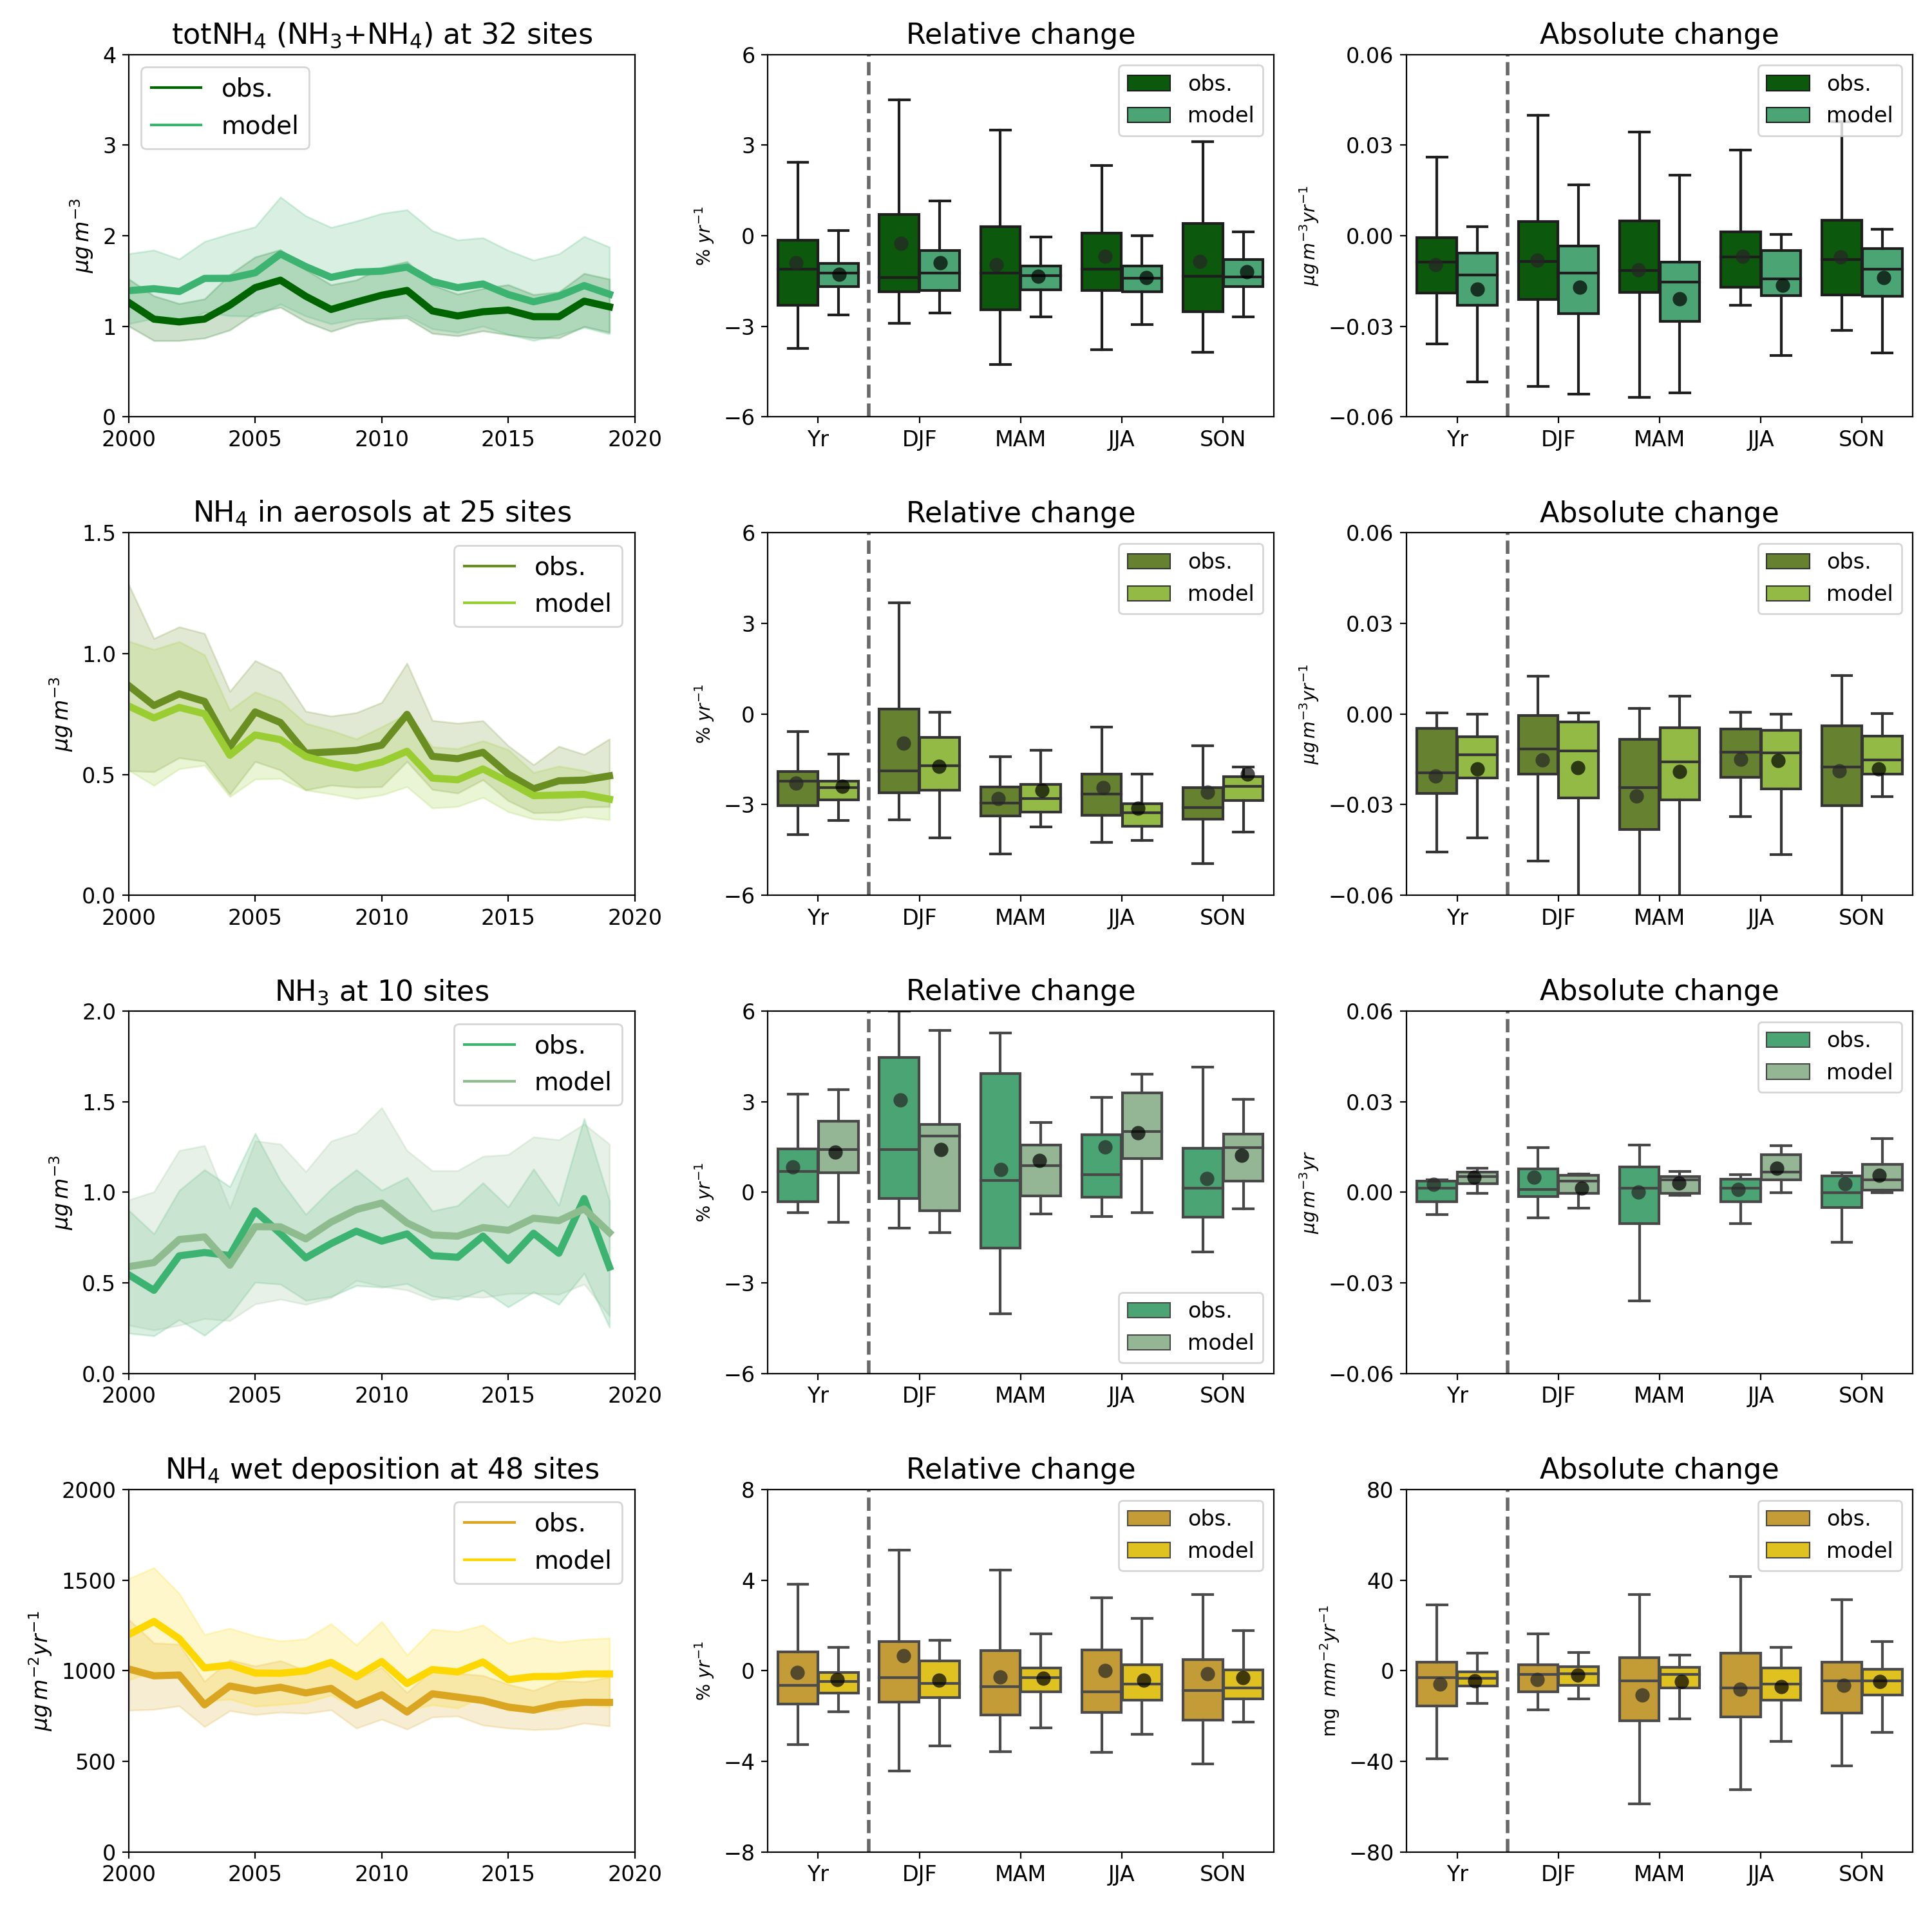
\includegraphics[width=0.74\paperwidth]{FIGS_TRENDS/Nred_trends.png}
	\caption{\label{fig:Nred_trends}Trends in oxidised nitrogen components from 2010-2019 for EMEP observations and model.}
\end{figure}



\begin{table}
\caption{\label{tab:tno3_stat} Average absolute and relative changes in  concentration of total ammonium (\nhiii+\nhiv) in air and aerosols}
\begin{center}
\scalebox{0.65}{%
\begin{tabular}{ll|ccc|cccc|cccc}
\toprule
          &        & \multicolumn{3}{c}{Number of sites} & \multicolumn{4}{c}{Average change per year (\ug $yr^{-1})$} & \multicolumn{4}{c}{Relative change per year (\% $yr^{-1}$)} \\
Period & Seasons &           total & sign.(obs.) & sign.(mod.) &                    obs. &          conf.interval &  mod. &          conf.interval &                     obs. &         conf.interval &  mod. &        conf.interval \\
\midrule
2000-2019 & all &              32 &          18 &          21 &                  -0.010 &  (-0.018, -0.001) & -0.018 &  (-0.024, -0.012) &                    -0.90 &    (-1.51, -0.3) & -1.28 &  (-1.49, -1.06) \\
          & autumn &              31 &          12 &           8 &                  -0.007 &   (-0.016, 0.003) & -0.014 &   (-0.02, -0.008) &                    -0.84 &   (-1.62, -0.06) & -1.20 &   (-1.49, -0.9) \\
          & spring &              32 &          10 &          19 &                  -0.011 &  (-0.021, -0.001) & -0.021 &  (-0.028, -0.013) &                    -0.95 &   (-1.65, -0.25) & -1.34 &  (-1.58, -1.09) \\
          & summer &              32 &          11 &          24 &                  -0.007 &   (-0.015, 0.002) & -0.016 &   (-0.023, -0.01) &                    -0.68 &   (-1.32, -0.04) & -1.39 &  (-1.62, -1.16) \\
          & winter &              35 &          11 &          13 &                  -0.008 &    (-0.02, 0.004) & -0.017 &  (-0.027, -0.007) &                    -0.26 &    (-1.03, 0.52) & -0.90 &  (-1.46, -0.33) \\
2005-2019 & all &              35 &          17 &          14 &                  -0.021 &  (-0.031, -0.011) & -0.017 &  (-0.025, -0.008) &                    -1.68 &    (-2.27, -1.1) & -1.01 &  (-1.97, -0.05) \\
2010-2019 & all &              35 &           9 &           9 &                  -0.015 &  (-0.024, -0.006) & -0.023 &    (-0.055, 0.01) &                    -1.82 &   (-2.68, -0.97) & -0.71 &   (-1.74, 0.33) \\
2000-2010 & all &              46 &           8 &          16 &                   0.000 &   (-0.018, 0.019) & -0.022 &   (-0.03, -0.014) &                     1.83 &    (-0.68, 4.35) & -1.13 &   (-1.7, -0.56) \\
\bottomrule
\end{tabular}}
\end{center}
\end{table}

\begin{table}
\caption{\label{tab:nh4pm_stat} Average absolute and relative changes in \nhiv concentrations in aerosols}
\begin{center}
\scalebox{0.65}{%
\begin{tabular}{ll|ccc|cccc|cccc}
\toprule
          &        & \multicolumn{3}{c}{Number of sites} & \multicolumn{4}{c}{Average change per year (\ug $yr^{-1})$} & \multicolumn{4}{c}{Relative change per year (\% $yr^{-1}$)} \\
Period & Seasons &           total & sign.(obs.) & sign.(mod.) &                    obs. &          conf.interval &  mod. &          conf.interval &                     obs. &         conf.interval &  mod. &        conf.interval \\
\midrule
2000-2019 & all &              25 &          16 &          22 &                  -0.021 &  (-0.029, -0.013) & -0.018 &  (-0.024, -0.012) &                    -2.29 &  (-2.78, -1.81) & -2.40 &  (-2.66, -2.13) \\
          & autumn &              23 &          12 &          12 &                  -0.019 &  (-0.026, -0.011) & -0.018 &   (-0.027, -0.01) &                    -2.58 &  (-3.39, -1.76) & -1.99 &  (-3.05, -0.93) \\
          & spring &              24 &          19 &          18 &                  -0.027 &  (-0.037, -0.017) & -0.019 &  (-0.026, -0.012) &                    -2.80 &  (-3.38, -2.23) & -2.53 &   (-2.96, -2.1) \\
          & summer &              24 &          14 &          22 &                  -0.015 &    (-0.02, -0.01) & -0.015 &    (-0.02, -0.01) &                    -2.43 &  (-3.05, -1.82) & -3.12 &  (-3.49, -2.76) \\
          & winter &              26 &          11 &           9 &                  -0.015 &   (-0.03, -0.001) & -0.018 &  (-0.025, -0.011) &                    -0.96 &   (-1.95, 0.04) & -1.73 &  (-2.17, -1.28) \\
2005-2019 & all &              33 &          16 &          24 &                  -0.020 &  (-0.028, -0.012) & -0.019 &  (-0.024, -0.013) &                    -2.37 &   (-3.34, -1.4) & -2.62 &  (-3.07, -2.16) \\
2010-2019 & all &              38 &          18 &          17 &                  -0.023 &  (-0.034, -0.012) & -0.016 &   (-0.023, -0.01) &                    -3.12 &  (-4.56, -1.67) & -2.57 &  (-3.36, -1.78) \\
2000-2010 & all &              30 &          11 &          13 &                  -0.026 &  (-0.039, -0.014) & -0.028 &  (-0.037, -0.018) &                    -2.03 &   (-4.27, 0.21) & -2.86 &   (-3.3, -2.41) \\
\bottomrule
\end{tabular}}
\end{center}
\end{table}

\begin{table}
\caption{\label{tab:nh3_stat} Average absolute and relative changes in \nhiii concentrations}
\begin{center}
\scalebox{0.65}{%
\begin{tabular}{ll|ccc|cccc|cccc}
\toprule
          &        & \multicolumn{3}{c}{Number of sites} & \multicolumn{4}{c}{Average change per year (\ug $yr^{-1})$} & \multicolumn{4}{c}{Relative change per year (\% $yr^{-1}$)} \\
Period & Seasons &           total & sign.(obs.) & sign.(mod.) &                    obs. &          conf.interval &  mod. &          conf.interval &                     obs. &         conf.interval &  mod. &        conf.interval \\
\midrule
2000-2019 & all &              10 &           2 &           6 &                   0.003 &  (-0.013, 0.019) &  0.005 &  (-0.004, 0.014) &                     0.85 &     (-0.6, 2.3) &  1.32 &    (0.46, 2.19) \\
          & autumn &              10 &           1 &           4 &                   0.003 &  (-0.009, 0.015) &  0.006 &  (-0.001, 0.012) &                     0.46 &   (-0.75, 1.67) &  1.22 &    (0.49, 1.94) \\
          & spring &              10 &           4 &           2 &                   0.000 &  (-0.021, 0.021) &  0.003 &   (-0.004, 0.01) &                     0.76 &   (-1.34, 2.86) &  1.05 &    (0.06, 2.04) \\
          & summer &              10 &           2 &           6 &                   0.001 &  (-0.024, 0.026) &  0.008 &  (-0.001, 0.016) &                     1.49 &   (-1.16, 4.15) &  1.97 &    (0.97, 2.97) \\
          & winter &              10 &           1 &           5 &                   0.005 &  (-0.002, 0.012) &  0.001 &  (-0.006, 0.009) &                     3.06 &    (0.08, 6.03) &  1.42 &    (0.06, 2.78) \\
2005-2019 & all &              23 &           4 &          10 &                   0.005 &  (-0.003, 0.013) &  0.001 &  (-0.007, 0.009) &                     0.31 &    (-0.49, 1.1) &  1.24 &    (0.11, 2.38) \\
2010-2019 & all &              29 &           4 &          10 &                   0.015 &  (-0.001, 0.032) &  0.004 &   (-0.012, 0.02) &                     3.50 &   (-0.02, 7.02) &  5.29 &  (-0.57, 11.15) \\
2000-2010 & all &              17 &           4 &           7 &                  -0.006 &  (-0.041, 0.028) &  0.016 &    (0.002, 0.03) &                     2.85 &    (0.29, 5.41) &  1.73 &    (0.27, 3.18) \\
\bottomrule
\end{tabular}}
\end{center}
\end{table}


\begin{table}
\caption{\label{tab:nh4dep_stat} Average absolute and relative changes in wet deposition of ammonium}
\begin{center}
\scalebox{0.7}{%
\begin{tabular}{ll|ccc|cccc|cccc}
\toprule
          &        & \multicolumn{3}{c}{Number of sites} & \multicolumn{4}{c}{Average change per year (mg $mm^{2} yr^{-1})$} & \multicolumn{4}{c}{Relative change per year (\% $yr^{-1}$)} \\
Period & Seasons &           total & sign.(obs.) & sign.(mod.) &                    obs. &          conf.interval &  mod. &          conf.interval &                     obs. &         conf.interval &  mod. &        conf.interval \\
\midrule
2000-2019 & all &              48 &          14 &           8 &                    -5.9 &  (-10.2, -1.5) &  -4.5 &   (-7.5, -1.4) &                    -0.07 &    (-0.73, 0.6) & -0.40 &  (-0.69, -0.11) \\
          & autumn &              47 &          10 &           5 &                    -6.3 &  (-11.3, -1.4) &  -4.8 &   (-8.6, -1.0) &                    -0.15 &   (-1.08, 0.79) & -0.32 &   (-0.77, 0.13) \\
          & spring &              46 &           5 &           4 &                   -10.9 &  (-17.7, -4.1) &  -4.9 &   (-11.1, 1.2) &                    -0.28 &    (-0.95, 0.4) & -0.32 &   (-0.68, 0.04) \\
          & summer &              47 &          10 &           5 &                    -8.1 &  (-14.3, -2.0) &  -7.0 &  (-10.4, -3.7) &                     0.01 &    (-0.98, 1.0) & -0.41 &  (-0.76, -0.07) \\
          & winter &              49 &           5 &           1 &                    -3.9 &   (-7.8, -0.0) &  -1.9 &    (-3.8, 0.1) &                     0.65 &   (-0.76, 2.06) & -0.42 &  (-0.73, -0.11) \\
2005-2019 & all &              56 &          10 &           4 &                    -3.4 &    (-9.1, 2.3) &  -3.0 &   (-5.9, -0.2) &                     1.40 &   (-1.43, 4.23) & -0.39 &  (-0.73, -0.05) \\
2010-2019 & all &              69 &           4 &           4 &                    -2.9 &   (-11.8, 5.9) &  -3.7 &    (-9.0, 1.5) &                     1.25 &    (-0.51, 3.0) & -0.09 &   (-0.73, 0.55) \\
2000-2010 & all &              52 &           6 &           3 &                    -4.8 &   (-13.5, 4.0) &  -2.1 &    (-9.4, 5.2) &                     0.03 &   (-1.07, 1.13) &  0.07 &   (-0.69, 0.83) \\
\bottomrule
\end{tabular}}
\end{center}
\end{table}



\section{\label{sec:Trends_PM }Trends in \PM[10] and \PM[2.5] }

Figure~\ref{fig:pm_trends} shows an overview of the annual and seasonal trends in \PM[10] and \PM[2.5] from 2000 to 2019. Tables \ref{tab:pm10_stat} and \ref{tab:pm25_stat} provide further quantitative information regarding observed and modelled trends, i.e. the number of sites considered and those with significant trends, values of average absolute and relative trends (including confidence intervals) for the 2000-2019 period, for 2000-2010 and 2010-2019 sub-periods, and also for the 2005-2019 period.


\begin{figure}
	\centering
	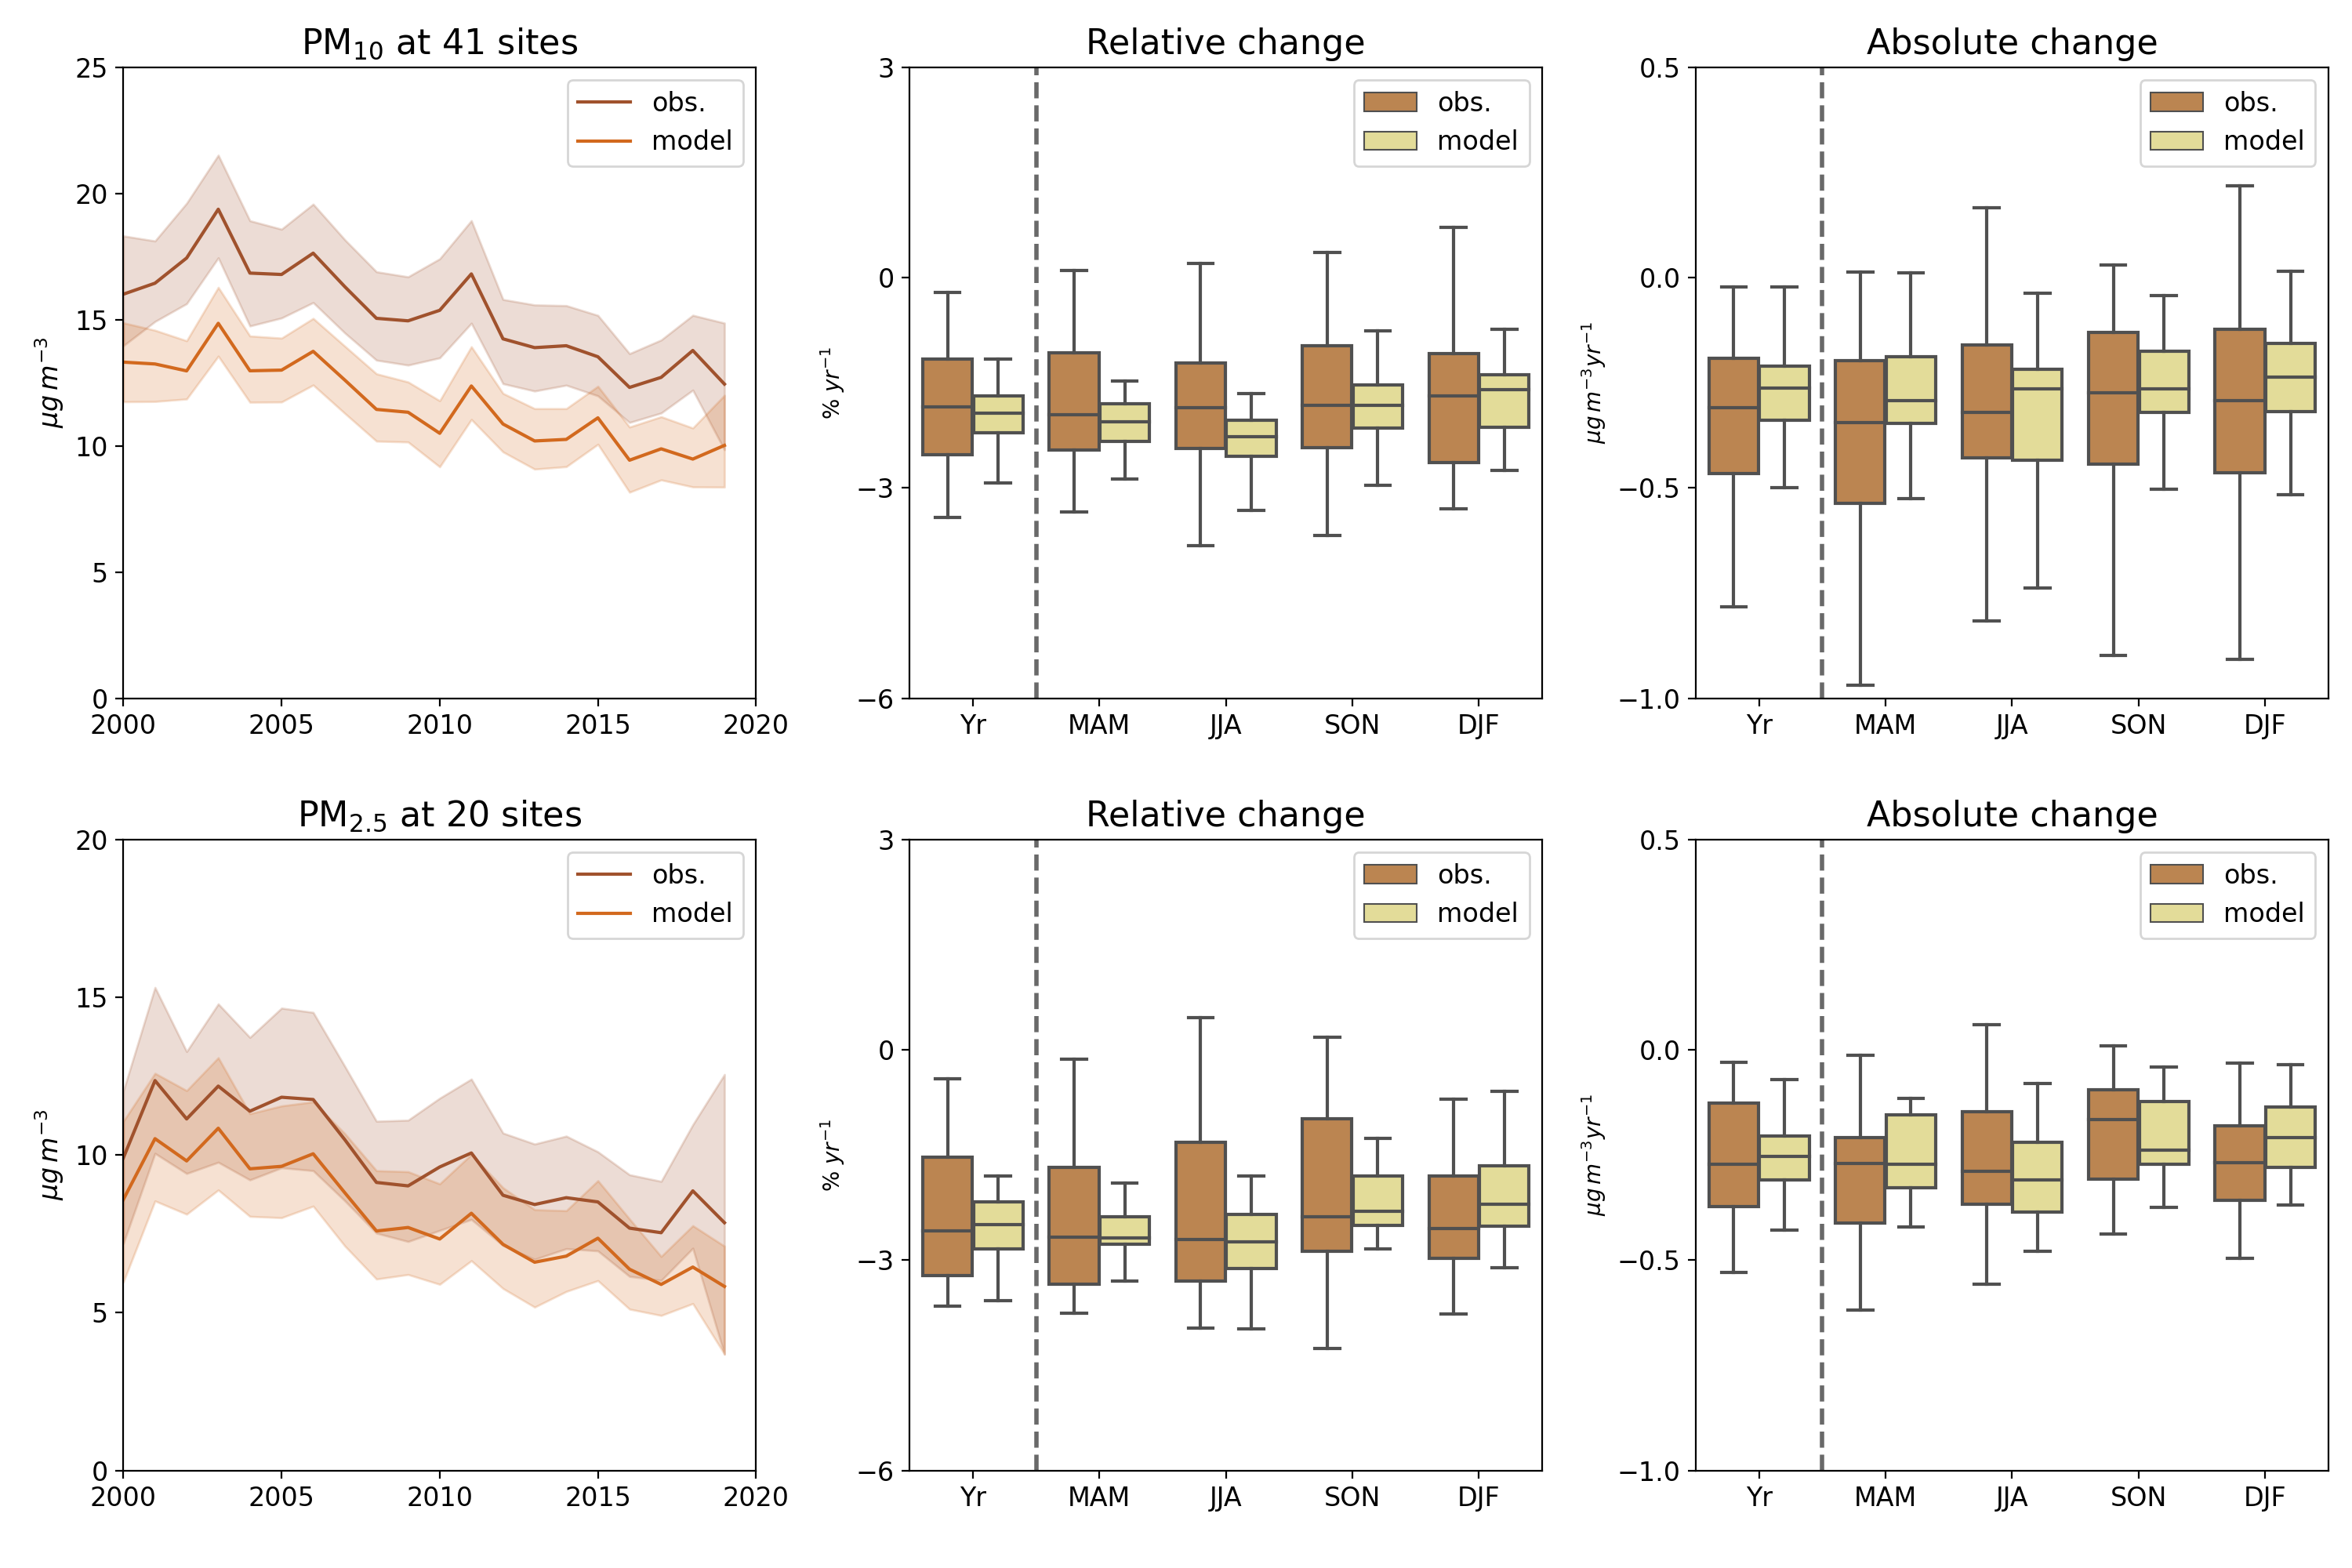
\includegraphics[width=0.74\paperwidth]{FIGS_TRENDS/PM_trends.png}
	\caption{\label{fig:pm_trends}Trends in \PM[10]  and \PM[2.5] from 2010-2019 for EMEP observations and model.}
\end{figure}


Overall, the model calculates significant PM trends at more sites 
In the period 2000-2019 for \PM[10] , 41 31 39 sites -0.35  -0.27 \ug $yr^{-1})$  -1.79  -1.95 \% $yr^{-1})$

For \PM[2.5] 20 16 20 sites -0.29  -0.25 ug $yr^{-1})$ -2.34  -2.52  \% $yr^{-1})$



\begin{table}
\caption{\label{tab:pm10_stat} Average absolute and relative changes in \PM[10]}
\begin{center}
\scalebox{0.65}{%
\begin{tabular}{ll|ccc|cccc|cccc}
\toprule
          &        & \multicolumn{3}{c}{Number of sites} & \multicolumn{4}{c}{Average change per year (\ug $yr^{-1})$} & \multicolumn{4}{c}{Relative change per year (\% $yr^{-1}$)} \\
Period & Seasons &           total & sign.(obs.) & sign.(mod.) &                    obs. &          conf.interval &  mod. &          conf.interval &                     obs. &         conf.interval &  mod. &        conf.interval \\
\midrule
2000-2019 & all &              41 &          31 &          39 &                   -0.35 &  (-0.42, -0.28) & -0.27 &   (-0.3, -0.23) &                    -1.82 &  (-2.06, -1.58) & -1.91 &  (-2.06, -1.76) \\
          & autumn &              38 &          23 &          30 &                   -0.33 &  (-0.41, -0.25) & -0.26 &   (-0.3, -0.23) &                    -1.83 &  (-2.12, -1.54) & -1.87 &  (-2.04, -1.69) \\
          & spring &              37 &          24 &          33 &                   -0.37 &   (-0.45, -0.3) & -0.28 &  (-0.32, -0.24) &                    -1.81 &  (-2.07, -1.56) & -2.05 &  (-2.24, -1.86) \\
          & summer &              39 &          28 &          33 &                   -0.33 &  (-0.41, -0.25) & -0.30 &  (-0.35, -0.24) &                    -1.70 &  (-2.05, -1.36) & -2.16 &  (-2.38, -1.94) \\
          & winter &              37 &          18 &          20 &                   -0.34 &  (-0.45, -0.24) & -0.25 &    (-0.3, -0.2) &                    -1.69 &   (-2.0, -1.38) & -1.57 &  (-1.81, -1.33) \\
2005-2019 & all &              58 &          31 &          38 &                   -0.32 &  (-0.39, -0.24) & -0.22 &  (-0.26, -0.18) &                    -1.80 &  (-2.19, -1.41) & -1.78 &  (-2.02, -1.53) \\
2010-2019 & all &              62 &          17 &          26 &                   -0.23 &  (-0.39, -0.07) & -0.16 &   (-0.2, -0.11) &                    -1.30 &  (-2.28, -0.33) & -1.35 &  (-1.74, -0.95) \\
2000-2010 & all &              39 &          15 &          24 &                   -0.47 &  (-0.56, -0.37) & -0.31 &   (-0.4, -0.22) &                    -2.42 &  (-2.81, -2.03) & -2.22 &  (-2.76, -1.68) \\
\bottomrule
\end{tabular}}
\end{center}
\end{table}

\begin{table}
\caption{\label{tab:pm25_stat} Average absolute and relative changes in \PM[25]}
\begin{center}
\scalebox{0.65}{%
\begin{tabular}{ll|ccc|cccc|cccc}
\toprule
          &        & \multicolumn{3}{c}{Number of sites} & \multicolumn{4}{c}{Average change per year (\ug $yr^{-1})$} & \multicolumn{4}{c}{Relative change per year (\% $yr^{-1}$)} \\
Period & Seasons &           total & sign.(obs.) & sign.(mod.) &                    obs. &          conf.interval &  mod. &          conf.interval &                     obs. &         conf.interval &  mod. &        conf.interval \\
\midrule
2000-2019 & all &              21 &          17 &          21 &                   -0.28 &  (-0.37, -0.19) & -0.24 &   (-0.29, -0.2) &                    -2.36 &  (-2.79, -1.94) & -2.47 &  (-2.66, -2.27) \\
          & autumn &              20 &          13 &          17 &                   -0.25 &  (-0.34, -0.15) & -0.23 &   (-0.3, -0.16) &                    -2.21 &  (-2.66, -1.76) & -2.21 &  (-2.44, -1.98) \\
          & spring &              21 &          15 &          20 &                   -0.31 &  (-0.39, -0.23) & -0.25 &   (-0.29, -0.2) &                    -2.42 &  (-2.88, -1.97) & -2.60 &    (-2.8, -2.4) \\
          & summer &              20 &          15 &          19 &                   -0.26 &  (-0.32, -0.19) & -0.28 &  (-0.34, -0.22) &                    -2.31 &  (-2.83, -1.79) & -2.73 &  (-3.04, -2.42) \\
          & winter &              20 &          13 &          15 &                   -0.34 &   (-0.5, -0.17) & -0.20 &  (-0.24, -0.16) &                    -2.24 &   (-2.69, -1.8) & -2.03 &  (-2.33, -1.73) \\
2005-2019 & all &              38 &          24 &          28 &                   -0.32 &  (-0.41, -0.23) & -0.20 &  (-0.24, -0.16) &                    -2.62 &  (-3.11, -2.12) & -2.23 &  (-2.48, -1.98) \\
2010-2019 & all &              45 &          21 &          19 &                   -0.33 &  (-0.41, -0.24) & -0.18 &  (-0.23, -0.13) &                    -3.02 &  (-3.61, -2.44) & -2.19 &  (-2.62, -1.76) \\
2000-2010 & all &              23 &           8 &          14 &                   -0.34 &  (-0.47, -0.21) & -0.33 &  (-0.41, -0.25) &                    -2.63 &  (-3.44, -1.82) & -2.92 &  (-3.49, -2.36) \\
\bottomrule
\end{tabular}}
\end{center}
\end{table}

\clearpage
\bibliographystyle{copernicus}         % change bibliography-name after each
\renewcommand\bibname{References}      % bibliographystyle command!
\addcontentsline{toc}{section}{References}
\bibliography{trends}

